\labelchapter{multiple-inheritance}{Multiple inheritance}

\index{classes!multiple inheritance}
Multiple inheritance is the ability to inherit from more than one superclass.  In OCaml, the
mechanism is simple, any class that contains more than one \hbox{\lstinline/inherit/} directive inherits
from each of them.

Object-oriented programming has received much attention over the years, and multiple inheritance is
one of the more controversial areas.  Some claims against it are that it is complicated, that it
requires extensive training to understand, or that all of its useful features can be captured with
interfaces.  Many of these claims are baloney---in fact, multiple inheritance is often one of the
simplest and most elegant way to combine features and abstractions.  However, there are two main
issues that give rise to these claims:

\begin{itemize}
\item \emph{shadowing}: what happens when two ancestor classes define a method with the same name?
\item \emph{repeated inheritance}: what happens when a class is inherited more than once?
\end{itemize}
%
As we will see, OCaml's model of inheritance is quite simple.  It is essentially equivalent to
textual inclusion, and shadowing follows the normal rule: if a method is defined more than once, the
last definition wins.  First though, let's turn to some examples.

\section{Examples of multiple inheritance}

Multiple inheritance arises whenever an object is described as a collection of features.  Examples
in the real world abound.

\begin{itemize}
\item A \emph{clock radio} is a \emph{timepiece} and a \emph{radio}.
\item An \emph{ambulance} is a \emph{vehicle} and an \emph{emergency medical facility}.
\item A \emph{mobile home} is a \emph{vehicle} and a \emph{home}.
\item A \emph{spork} is a \emph{spoon} and a \emph{fork}.
\item A \emph{graduate student} is a \emph{graduate} and a \emph{student}.
\item A \emph{Swiss army knife} is a \emph{knife} and \emph{scissors} and \emph{pliers} and a \emph{screwdriver} and...
\end{itemize}
%
If we consider these examples, there are really two kinds of combinations: those of independent
features like \emph{clock} and \emph{radio}; and those of related features.  For example, spoons and forks are
both utensils, graduates and students are kinds of persons, \emph{etc}.

\subsection{Inheriting from multiple independent classes}

From a programming perspective, inheritance from independent classes is simpler.  When the classes
to be combined use disjoint names, the result of combining them is simply to produce an object with
all the parts.  For example, consider the following sketches of the classes \hbox{\lstinline/clock/}
and \hbox{\lstinline/radio/}.

\begin{ocaml}
class clock =
object
   val mutable now = $\cdots$
   method gettimeofday = now
   method private tick = $\cdots$
end;;

class radio =
object
   val mutable frequency = 89.3e6
   val mutable volume = 11.0
   method tune freq = $\cdots$; frequency <- freq
   method set_volume vol = $\cdots$; volume <- vol
end;;
\end{ocaml}
%
The combined class \hbox{\lstinline/clock_radio/} simply inherits from both.  The resulting class has the
methods and fields of both superclasses.

\begin{ocaml}
# class clock_radio =
  object
     inherit clock
     inherit radio
  end;;
@
\begin{topoutput}
class clock_radio :
  object
    val mutable frequency : float
    val mutable now : float
    val mutable volume : float
    method gettimeofday : float
    method set_volume : float -> unit
    method private tick : unit
    method tune : float -> unit
  end
\end{topoutput}
@
\end{ocaml}

\subsection{Inheriting from multiple virtual classes}

Sometimes inheritance is used as a mechanism to add functionality by inheriting from a partially
virtual superclass.  Let's take a look at an example, based on the class \hbox{\lstinline/comparable/} we
introduced on page~\pageref{page:comparable}.  We'll define two virtual classes.

\begin{itemize}
\item A \hbox{\lstinline/comparable/} value can be compared to values of the same type.
\item \lstinline/number/ is a class of numbers that can be compared, having a zero, and a negation function.
\end{itemize}
%
The virtual class \hbox{\lstinline/comparable/} declares a virtual method \hbox{\lstinline/compare/}, and derives a
method \hbox{\lstinline/less_than/} from it.

\begin{ocaml}
(* less-than: negative; equal: zero; greater-than: positive *)
type comparison = int

class virtual comparable =
object (self : 'self)
   method virtual compare : 'self -> comparison
   method less_than (x : 'self) = compare self x < 0
end;;
\end{ocaml}
%
For the class \hbox{\lstinline/number/}, we require that the subclass provide
methods \hbox{\lstinline/zero/}, \hbox{\lstinline/neg/} (negate), and \hbox{\lstinline/compare/}.  From that, a
method \hbox{\lstinline/abs/} (absolute value) can be derived.

\begin{ocaml}
class virtual number =
object (self : 'self)
   method virtual zero : 'self
   method virtual neg : 'self
   method virtual compare : 'self -> comparison
   method abs =
      if self#compare self#zero < 0 then
         self#neg
      else
         self
end;;
\end{ocaml}
%
Finally, an actual concrete class of numbers inherits from both classes \hbox{\lstinline/comparable/}
and \hbox{\lstinline/number/}, implementing the virtual methods, and inheriting the derived methods.  The
following class also implements the methods \hbox{\lstinline/less_than/} and \hbox{\lstinline/abs/}
because it inherits them from the virtual superclasses.

\begin{ocaml}
class float_number x =
object (self : 'self)
   inherit comparable
   inherit number

   val number = x
   method representation = number
   method zero = {< number = 0.0 >}
   method neg = {< number = -. number >}
   method compare y = Pervasives.compare x y#representation
end;;
\end{ocaml}

\subsection{Mixins}

\index{mixins}
\index{classes!mixins}
\index{Steve's Ice Cream Parlor}
A \emph{mixin} is a class that is used to add augment the functionality of or
change the behavior of a subclass, but there is no explicit is-a relationship.  According to
folklore, the term mix-in was inspired by Steve's Ice Cream Parlor in Somerville, Massachusetts,
where extra items like nuts, chocolate sprinkles, \emph{etc}., were mixed into a base flavor of ice
cream like chocolate or vanilla.

Let's implement some ice cream with two arbitrary mixed-in flavors.  We'll use the drawable objects
of Chapter~\ref{chapter:objects1}.  A \hbox{\lstinline/blob/} is an object that can be drawn,
including the classes \hbox{\lstinline/circle/} and \hbox{\lstinline/poly/}, and a \hbox{\lstinline/collection/}
is a collection of blobs.

\begin{ocaml}
class vanilla_ice_cream = object $\cdots$ end

class virtual mixed_ice_cream =
object (self)
   inherit vanilla_ice_cream
   inherit collection

   method virtual mixin1 : unit
   method virtual mixin2 : unit

   method stir = self#map (fun item ->
      let t = recenter ** transform#new_rotate (Random.float 6.28)
         ** transform#new_translate (Random.float 10.) (sqrt (Random.float 1e4))
      in item#transform t)

   initializer self#mixin1; self#mixin2; self#stir
end
\end{ocaml}
%
Vanilla ice cream is featureless, but the mixed ice cream contains a collection of extra items.  The
virtual methods \hbox{\lstinline/mixin1/} and \hbox{\lstinline/mixin2/} add the extra items to the collection.  To
implement a particular kind of mixed ice cream, we implement two classes, one for each mixin.

\begin{ocaml}
class drop = circle ~color:0x880022 (0., 0.) 10.
class sprinkle = poly ~color:0x220044 [|(0., 0.); (10., 0.); (10., 3.); (0., 3.)|]

class virtual drop_mixin1 =
object (self)
   method virtual add : blob -> unit
   method mixin1 = for i = 0 to 4 do self#add (new drop) done
end

class virtual sprinkle_mixin2 =
object (self)
   method virtual add : blob -> unit
   method mixin2 = for i = 0 to 200 do self#add (new sprinkle) done
end
\end{ocaml}
%
For the final product, we just mix the ice cream with its ingredients.
The mixin classes implement the virtual methods of the ice cream class,
and the result is a flavored ice cream.

\begin{ocaml}
class my_favorite_ice_cream =
object
   inherit mixed_ice_cream
   inherit drop_mixin1
   inherit sprinkle_mixin2
end
\end{ocaml}
%
This use of inheritance is not a specialization.  We certainly don't mean
that \hbox{\lstinline/my_favorite_ice_cream/} is-a \hbox{\lstinline/sprinkle/}, or a collection of sprinkles, or
anything of the sort.  The purpose of the inheritance in this case is simply for the mixin to
specify an item that is to be added to the ice cream.

\begin{center}
\begin{tabular}{ll}
\begin{minipage}[b]{2in}
\begin{ocamllisting}
(new my_favorite_ice_cream)#draw;;
\end{ocamllisting}
\end{minipage}
&
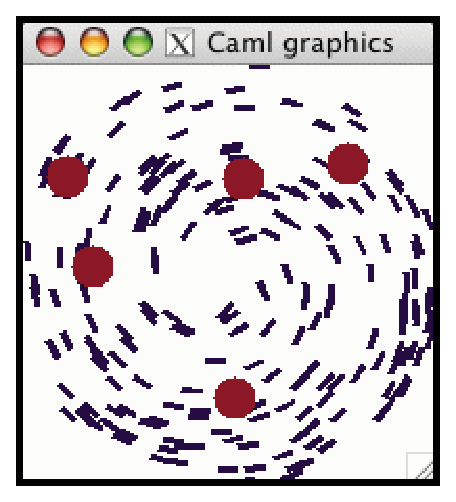
\includegraphics[scale=0.3]{ice_cream}
\end{tabular}
\end{center}
%
In all the examples of this section, the inheritance is used to combine classes that are
really independent.  In each case, there may be several declarations of a method as virtual, but there only
one implementation.  Let's turn to the more general case where methods and fields may be defined
multiple times, starting with the topic of \emph{shadowing}.

\section{Overriding and shadowing}

What happens when an object defines a name twice?  For comparison, let's first consider a similar
question: what happens in a module when a name is defined twice?  We know the answer---the
definition exported by the module is the last one.

\begin{ocaml}
# module M =
  struct
     let x = 1;;
     Printf.printf "x = %d!\n" x;;
     let x = 2;;
  end;;
@
\begin{topoutput}
x = 1!
\end{topoutput}
@
# M.x;;
@
\begin{topoutput}
- : int = 2
\end{topoutput}
@
\end{ocaml}
%
Objects are a little different from modules, but the naming is similar.  Consider the following
objects that contain duplicate definitions.  OCaml warns about the duplication, but it is
instructive to see the results.  First, let's override a method.

\begin{ocaml}
# let a =
  object
     method get = 1
     method get = 2
  end;;
@
\begin{topoutput}
Warning M: the method get is overriden in the same class.
val a : < get : int > = <obj>
\end{topoutput}
@
# a#get;;
- : int = 2
\end{ocaml}
%
As would be expected, the last method definition is the one that is used by the object.
We can try the same thing with fields.

\begin{ocaml}
# let b =
  object
     val x = 1
     method get = x
     val x = 2
  end;;
@
\begin{topoutput}
Warning V: the instance variable x is overriden.
\end{topoutput}
@
# b#get;;
@
\begin{topoutput}
- : int = 2
\end{topoutput}
@
\end{ocaml}
%
Field override seems to be frowned upon by the compiler.  Still, the result is the same, it is the
last definition that is used by the object.  Any preceding definitions for the same name are
ignored.

\section{Repeated inheritance}
\index{inheritance!repeated}
\index{inheritance!diamond problem}
\index{classes!repeated inheritance}
\index{classes!diamond problem}

Repeated inheritance occurs when a class inherits from another along multiple paths in the
inheritance hierarchy, perhaps more commonly known as the ``diamond problem.''  For example, we
might say that a French programmer is both French and a programmer, and both of these are more
generally persons.  That means that a French programmer inherits from person twice.  The following
diagram illustrates the class relationship, with a hypothetical programmer in italics.

\begin{center}
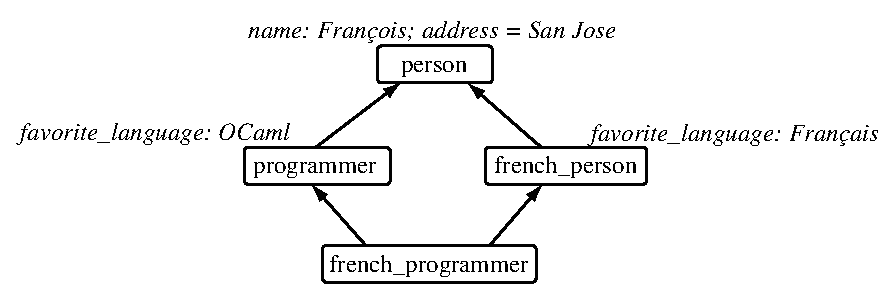
\includegraphics[scale=0.75]{french-programmer}
\end{center}
%
In OCaml, the \hbox{\lstinline/inherit/} directive is nearly equivalent to textual inclusion---the result
is the same as if the \hbox{\lstinline/inherit/} clause were replaced with the text of the class being
inherited from.  This means that a \hbox{\lstinline/programmer/} includes the program text for
a \hbox{\lstinline/person/}, so does a \hbox{\lstinline/french_person/}, and the \hbox{\lstinline/french_programmer/}
contains the program text twice.

When does this make a difference?  For any given method or field, remember the rule: it is
the \emph{last} definition that matters, so perform the textual expansion mentally and look for the
final definition.  Consider a case where a class \hbox{\lstinline/a/} is inherited twice.

\begin{ocamlnum}
# class a =
  object
     method x = 1
  end;;
# class b =
  object
     inherit a
     method x = 2
     inherit a
  end;;
@
\begin{topoutput}
Warning: ... x ... is overriden by the class a
\end{topoutput}
@
# (new b)#x;;
@
\begin{topoutput}
- : int = 1
\end{topoutput}
@
\end{ocamlnum}
%
The result is \hbox{\lstinline/1/} because the final definition for the method \hbox{\lstinline/x/} comes from the
inherit clause on line 9 (which defines \hbox{\lstinline/x/} as \hbox{\lstinline/1/}).

The diamond problem is similar.  Consider the French programmer example, here
drawn in the shape of a diamond (don't type it in this way).

\begin{center}
\begin{minipage}{4in}
\begin{ocamllisting}
                      class person =
                      object
                          method name = "Francois"
                          method address = "San Jose"
                      end

class programmer =                     class french_person =
object                                 object
   inherit person                         inherit person
   method lang = "OCaml"                  method lang = "Francais"
end                                    end

                      class french_programmer =
                      object
                          inherit programmer
                          inherit french_person
                      end
\end{ocamllisting}
\end{minipage}
\end{center}
%
Let's think how the text will be expanded for class \hbox{\lstinline/french_programmer/}.  If we perform the expansion,
here is the order in which the methods are defined:
\hbox{\lstinline/person#name,address/}, \hbox{\lstinline/programmer#lang/}, \hbox{\lstinline/person#name,address/}, \hbox{\lstinline/french_person#lang/}.
Keeping only the final definition for each method, we obtain the following class,
equivalent to \hbox{\lstinline/french_programmer/}.

\begin{ocaml}
class french_programmer_flattened =
object
   method name = "Francois"
   method lang = "Francais"
   method address = "San Jose"
end
\end{ocaml}
%
Field override works the same as method override for fields that are visible.  If we had defined the
values as fields instead of methods, the result would be the same: the
favorite language is Fran\c{c}ais.

However, fields that are hidden (because of typing) are not overridden; they are duplicated.
Suppose we define a class \hbox{\lstinline/a/} that defines a mutable field \hbox{\lstinline/x/}, which is then
hidden using a type constraint.

\begin{ocaml}
class type a_type =
object
   method set : int -> unit
   method get : int
end;;

class a : a_type =
object
   val mutable x = 0
   method set y = x <- y
   method get = x
end;;
\end{ocaml}
%
Repeated inheritance \emph{duplicates} the hidden field \hbox{\lstinline/x/}, which means that operations
on one copy of \hbox{\lstinline/a/} do not effect the others.

\begin{ocaml}
# class b =
  object
     inherit a as super1
     inherit a as super2

     method test =
        super1#set 10;
        super2#get
  end;;
@
\begin{topoutput}
class b :
  object method get : int method set : int -> unit method test : int end
\end{topoutput}
@
# (new b)#test;;
@
\begin{topoutput}
- : int = 0
\end{topoutput}
@
\end{ocaml}

\section{Avoiding repeated inheritance}

The previous section points out the issue with multiple inheritance, which is that there
are at least two different policies for repeated inheritance: override and copying.
There is no single policy that is best.  For example, the French programmer
may wish to go by the same name in all contexts, but he might wish to use a different address for
his occupation than he uses as a French citizen.  That is, the repeated field \hbox{\lstinline/name/}
should refer to the same value, but the \hbox{\lstinline/address/} field should be copied.

As pointed out, OCaml uses the following policy: visible fields and methods use the override policy,
fields and methods that are hidden use the copy policy.  This policy can be difficult for a
programmer to adhere to, ``All the fields that are hidden are copied.''  The semantics of multiple
inheritance might be simple enough to state, ``it is just textual expansion,'' but the problem is
that it might be necessary to know the text of all repeated superclasses.  For this reason and
others, it is natural to want to avoid repeated inheritance, at least in some cases.

\subsection{Is-a \emph{vs}.{} has-a}

For an example, suppose we have classified vehicles in two different ways: according to where they
are used, and by how they are powered.  In the following diagram, the class \hbox{\lstinline/vehicle/} is a
superclass of all the others; for example it might contain methods to move forward or
stop, \emph{etc}.  A \hbox{\lstinline/car/} is a vehicle that travels roads, a \hbox{\lstinline/boat/} water;
an \hbox{\lstinline/electric_vehicle/} needs to be charged occasionally, \emph{etc}.

\begin{center}
\begin{tabular}{|c|c|}
\hline
\multicolumn{2}{|c|}{\hbox{\lstinline/vehicle/}}\\
\hline
\hbox{\lstinline/car/} & \hbox{\lstinline/electric_vehicle/}\\
\hbox{\lstinline/boat/} & \hbox{\lstinline/gasoline_vehicle/}\\
\hbox{\lstinline/submarine/} & \hbox{\lstinline/rocket/}\\
\hbox{\lstinline/spacecraft/} & \hbox{\lstinline/pedaled_vehicle/}\\
& \hbox{\lstinline/sailed_vehicle/}\\
& \hbox{\lstinline/nuclear_vehicle/}\\
\hline
\end{tabular}
\end{center}
%
A particular kind of vehicle can constructed by combining a property from the left column and
another from the right.  We have gasoline powered boats, nuclear submarines, and electric cars.
Some combinations don't make much sense, like pedaled spacecraft.

On the surface, this classification may seem reasonable.  We classify vehicles by two
orthogonal properties, and use multiple inheritance to define classes for the combinations that make
sense.  However, this will involve repeated inheritance, which might be a problem if we don't know how
the class \hbox{\lstinline/vehicle/} is defined.

There is another way to classify vehicles that is just as natural, but avoids the repeated
inheritance.  That is, we can continue to classify vehicles by where they travel, but instead of
classifying powered vehicles, we classify power sources directly.

\begin{center}
\begin{tabular}{lr}
\begin{tabular}[t]{|c|}
\hline
\hbox{\lstinline/vehicle/}\\
\hline
\hbox{\lstinline/car/}\\
\hbox{\lstinline/boat/}\\
\hbox{\lstinline/submarine/}\\
\hbox{\lstinline/spacecraft/}\\
\hline
\end{tabular}
&
\begin{tabular}[t]{|c|}
\hline
\hbox{\lstinline/power_source/}\\
\hline
\hbox{\lstinline/electric_motor/}\\
\hbox{\lstinline/gasoline_engine/}\\
\hbox{\lstinline/rocket_engine/}\\
\hbox{\lstinline/pedals/}\\
\hbox{\lstinline/sails/}\\
\hbox{\lstinline/nuclear_plant/}\\
\hline
\end{tabular}
\\
\multicolumn{2}{c}{
\begin{tabular}[t]{|c|}
\hline
\hbox{\lstinline/assembled_vehicle/}\\
\hline
\hbox{\lstinline/electric_car = car + electric_motor/}\\
\hbox{\lstinline/nuclear_submarine = submarine + nuclear_plant/}\\
\hbox{\lstinline/sailboat = boat + sails/}\\
\hbox{\lstinline/rocket = spacecraft + rocket_engine/}\\
$\cdots$\\
\hline
\end{tabular}}
\end{tabular}
\end{center}
%
Now we have two independent concepts, vehicles and power sources, and an assembled vehicle needs one
of each.  The assemblies can be created with multiple inheritance, which has the advantage that
bogus assemblies (like rocket-powered submarines) can be omitted from the collection.

An alternative to multiple inheritance is for the vehicle class to take a power source as an
argument and include it as a field.  There are two potential advantages.  One is
that it is not necessary to write down every possible assembly.  The other is that it might make
more sense semantically---a vehicle has-a power source, but it isn't-a power source, at least not
normally.  A disadvantage is that it isn't easy to rule out combinations that don't make sense.

\subsection{Mixins revisited}

In many ways, the approach to the vehicle example is really just a mixin.  Power sources aren't
really useful until they are harnessed, which happens when an assembled vehicle is created by mixing
in a power source into a vehicle.

This suggests that one approach to avoiding repeated inheritance is to delay the use of multiple
inheritance as much as possible.  Returning to the French programmer, there were four classes with a
repeated base class \hbox{\lstinline/person/}.  Another way to design the hierarchy is to partition the
properties, where the programming and French properties are split from the \hbox{\lstinline/person/} and
become mixins.

\begin{center}
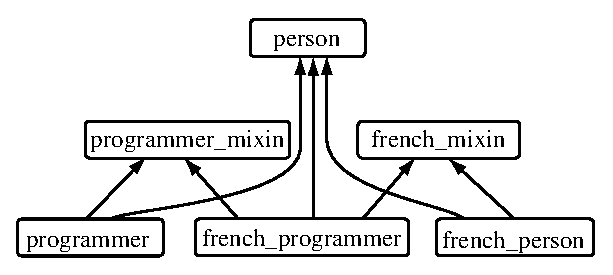
\includegraphics[scale=0.75]{french-mixin}
\end{center}
%
The mixin classes \hbox{\lstinline/programmer_mixin/} and \hbox{\lstinline/french_mixin/} are now standalone
classes.  They can still refer to the properties of being a person through virtual methods and fields, but they
don't make much sense alone until combined with the \hbox{\lstinline/person/} class.

As with any programming style, it isn't always appropriate to program this way.  There are more
classes; the relationship between classes is not as well defined---there is nothing that says that
a \hbox{\lstinline/programmer_mixin/} is to be combined with a \hbox{\lstinline/person/}; and it is easy to forget
about maintaining the relationship between a class and its mixins.  Of course, in many cases
this \emph{is} a useful technique, and it can lead to simpler, shorter programs.

At this point we have covered objects, classes with single inheritance, and classes with multiple
inheritance.  The object system is quite powerful, and we have many tools at our disposal.  There is
one remaining important topic: polymorphic classes, which we discuss in the next chapter.

% -*-
% Local Variables:
% Mode: LaTeX
% fill-column: 100
% TeX-master: "paper"
% TeX-command-default: "LaTeX/dvips Interactive"
% End:
% -*-
% vim:tw=100:fo=tcq:
